\section{Prof. Chapdelains kontor}
\label{loc:ChapdelainsKontor}
%
\begin{figure}[h]
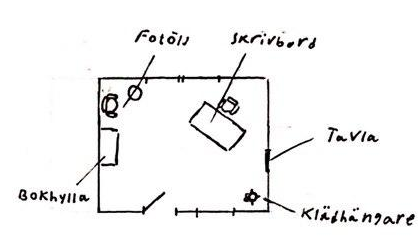
\includegraphics[width=8cm]{ProfChapsKontor.png}
\centering
\end{figure}
%
Professor Chapdelains är för närvarande inte på sitt kontor, men utredarna kan lätt upptäcka att dörren är olåst. Kontoret verkar vara mycket spartanskt. Det finns en tom bokhylla, ett skrivbord, en kontorsstol samt ett konstverk.

\begin{displayquote}
	Tavlan föreställer ett lila moln, eller kanske en vortex, som verkar strömma ut ur målningen. I botten på tavlan kan man se siluetter av människor som verkar utföra någon form av ceremoni eller tillbedjan. Verket är omslutet av en mörk träram.
\end{displayquote}

\begin{displayquote}
	Skrivbordet är en massiv pjäs i mörkt trä, med en tillhörande kontorsstol. Det står ut mot rummet, och är tomt.
\end{displayquote}
%
Med ett normalt lyckat slag emot intelligens inser utredarna att både skrivbordet och bokhyllan är täckta i ett tjockt lager damm. Om utredarna kollar i en av de två skrivbordslådorna hittar de där en gammal bibel. Om utredarna vill undersöka bokhyllan så är den för hög för att man ska kunna se ovansidan, så de behöver antingen assistans från en annan utredare, eller något att stå på för att göra en genomgående undersökning. Lyckas denne slå ett lyckat svårt slag för finna dolda ting när de kan se hela bokhyllan hittar de en bit tejp på den översta hyllan som verkar fästa i någonting på baksidan av bokhyllan. Med ett lyckat normalt slag för fingerfärdighet kan de fiska upp den lapp som sitter på baksidan av bokhyllan. De kan även försöka flytta bokhyllan med ett normalt lyckat slag, och på så sätt få tag i lappen. Lappen är densamme som Migele har i rockfickan när de träffar på honom på Brådmans Bar \sectiondescribe{\ref{loc:BradmansBar}}.
